\documentclass[aspectratio=169,12pt]{beamer}
\usepackage[utf8]{inputenc}
\usepackage{amsmath, amssymb}
\usepackage{booktabs}
\usepackage{colortbl}
\usepackage{hyperref}
\usepackage{makecell}
\usepackage{ragged2e}
\usepackage{bytefield}
\usepackage{tikz}
\usetikzlibrary{arrows.meta, positioning, shapes.geometric, calc, tikzmark, shapes.misc, matrix, decorations.pathreplacing, backgrounds}
\usepackage{tcolorbox}
\usetheme{Madrid}
\title{Multithreading and Power}
\author{Computer Architecture 2360267}
\date{2025, Recitation \#12}

\begin{document}

\frame{\titlepage}

\begin{frame}{Outline}
\tableofcontents
\end{frame}

\section{Execution Models and Multithreading}

\begin{frame}{Scalar Execution}
\begin{itemize}
    \item Sequential execution of instructions
    \item One instruction at a time
    \item Dependencies reduce throughput/utilization
\end{itemize}

\vspace{0.5cm}
\begin{center}
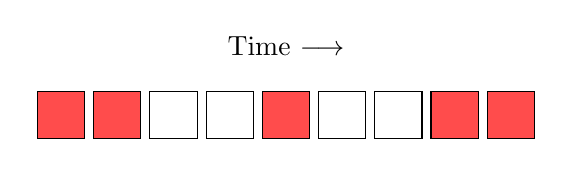
\begin{tikzpicture}[scale=0.5,
    filled/.style={fill=red!70},
    empty/.style={fill=white}]
    \matrix[matrix of nodes,
        nodes={draw=black, minimum size=6mm, anchor=center},
        column sep=1mm, row sep=1mm,
        ampersand replacement=\&] (m) {
        |[filled]| \phantom{X} \& |[filled]| \phantom{X} \& |[empty]| \phantom{X} \& |[empty]| \phantom{X} \& |[filled]| \phantom{X} \& |[empty]| \phantom{X} \& |[empty]| \phantom{X} \& |[filled]| \phantom{X} \& |[filled]| \phantom{X} \\
    };
    \node[above=2mm of m.north] {Time $\longrightarrow$};
\end{tikzpicture}
\end{center}

\begin{alertblock}{Key Issue}
Dependencies reduce throughput/utilization
\end{alertblock}
\end{frame}

\begin{frame}{Superscalar Execution}
\begin{columns}
\column{0.45\textwidth}
\begin{itemize}
    \item Multiple instructions per cycle
    \item Out-of-order execution capabilities
    \item Still limited by:
    \begin{itemize}
        \item Dependencies
        \item Cache misses
        \item Branch mispredictions
    \end{itemize}
\end{itemize}

\column{0.55\textwidth}
\begin{center}
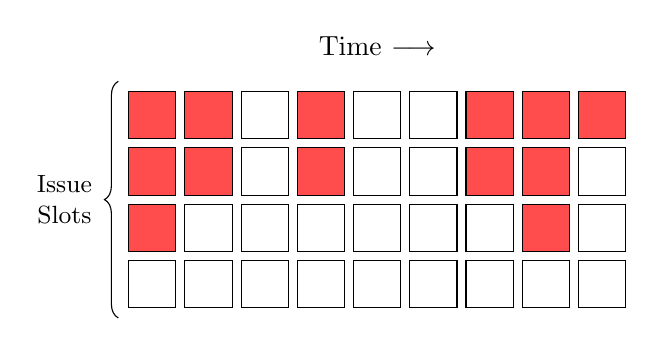
\begin{tikzpicture}[scale=0.5,
    filled/.style={fill=red!70},
    empty/.style={}]
    \matrix[matrix of nodes,
        nodes={draw=black, minimum size=6mm, anchor=center},
        column sep=1mm, row sep=1mm,
        ampersand replacement=\&] (m) {
        |[filled]| \phantom{X} \& |[filled]| \phantom{X} \& \phantom{X} \& |[filled]| \phantom{X} \& \phantom{X} \& \phantom{X} \& |[filled]| \phantom{X} \& |[filled]| \phantom{X} \& |[filled]| \phantom{X} \\
        |[filled]| \phantom{X} \& |[filled]| \phantom{X} \& \phantom{X} \& |[filled]| \phantom{X} \& \phantom{X} \& \phantom{X} \& |[filled]| \phantom{X} \& |[filled]| \phantom{X} \& \phantom{X} \\
        |[filled]| \phantom{X} \& \phantom{X} \& \phantom{X} \& \phantom{X} \& \phantom{X} \& \phantom{X} \& \phantom{X} \& |[filled]| \phantom{X} \& \phantom{X} \\
        \phantom{X} \& \phantom{X} \& \phantom{X} \& \phantom{X} \& \phantom{X} \& \phantom{X} \& \phantom{X} \& \phantom{X} \& \phantom{X} \\
    };
    \node[above=2mm of m.north] {Time $\longrightarrow$};
    \draw[decorate, decoration={brace, amplitude=5pt, mirror}]
        (m.north west) -- (m.south west)
        node[midway, left=6pt, font=\small, align=center] {Issue\\Slots};
\end{tikzpicture}
\end{center}
\end{columns}

\begin{alertblock}{Key Issue}
Dependencies, cache misses, and branch mispredictions reduce throughput/utilization
\end{alertblock}
\end{frame}

\begin{frame}{Blocked Multithreading}
\framesubtitle{Switch on Event}

\begin{columns}
\column{0.45\textwidth}
\begin{itemize}
    \item Switch threads when current thread encounters low utilization event
    \item Examples of switching events:
    \begin{itemize}
        \item L2 cache miss
        \item Long latency operations
    \end{itemize}
    \item May increase utilization and throughput
\end{itemize}

\column{0.55\textwidth}
\begin{center}
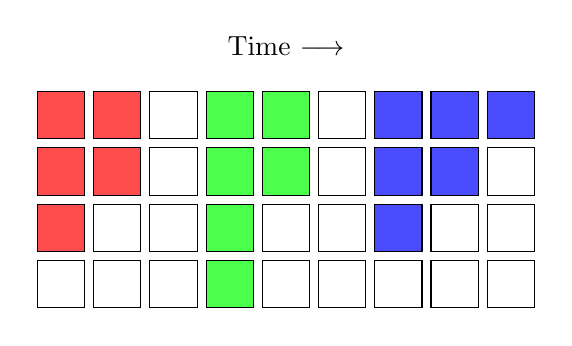
\begin{tikzpicture}[scale=0.5,
    T0/.style={fill=red!70},
    T1/.style={fill=green!70},
    T2/.style={fill=blue!70}]
    \matrix[matrix of nodes,
        nodes={draw=black, minimum size=6mm, anchor=center},
        column sep=1mm, row sep=1mm,
        ampersand replacement=\&] (m) {
        |[T0]| \phantom{X} \& |[T0]| \phantom{X} \& \phantom{X} \& |[T1]| \phantom{X} \& |[T1]| \phantom{X} \& \phantom{X} \& |[T2]| \phantom{X} \& |[T2]| \phantom{X} \& |[T2]| \phantom{X} \\
        |[T0]| \phantom{X} \& |[T0]| \phantom{X} \& \phantom{X} \& |[T1]| \phantom{X} \& |[T1]| \phantom{X} \& \phantom{X} \& |[T2]| \phantom{X} \& |[T2]| \phantom{X} \& \phantom{X} \\
        |[T0]| \phantom{X} \& \phantom{X} \& \phantom{X} \& |[T1]| \phantom{X} \& \phantom{X} \& \phantom{X} \& |[T2]| \phantom{X} \& \phantom{X} \& \phantom{X} \\
        \phantom{X} \& \phantom{X} \& \phantom{X} \& |[T1]| \phantom{X} \& \phantom{X} \& \phantom{X} \& \phantom{X} \& \phantom{X} \& \phantom{X} \\
    };
    \node[above=2mm of m.north] {Time $\longrightarrow$};
\end{tikzpicture}
\end{center}
\end{columns}

\begin{block}{Benefit}
Hides long latency events by switching to another thread
\end{block}
\end{frame}

\begin{frame}{Fine Grained Multithreading}
\begin{columns}
\column{0.45\textwidth}
\begin{itemize}
    \item Switch threads frequently (e.g., every cycle)
    \item Reduces impact of dependencies
    \item Better latency hiding than blocked multithreading
\end{itemize}

\column{0.55\textwidth}
\begin{center}
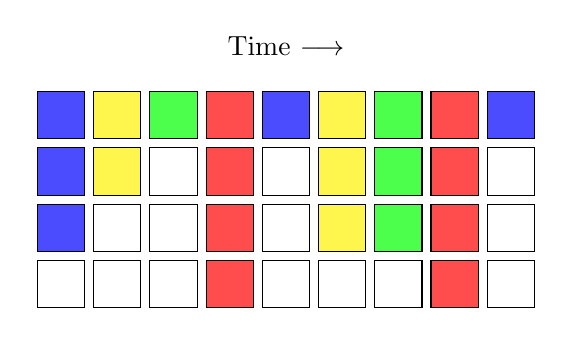
\begin{tikzpicture}[scale=0.5,
    T0/.style={fill=blue!70},
    T1/.style={fill=yellow!70},
    T2/.style={fill=green!70},
    T3/.style={fill=red!70}]
    \matrix[matrix of nodes,
        nodes={draw=black, minimum size=6mm, anchor=center},
        column sep=1mm, row sep=1mm,
        ampersand replacement=\&] (m) {
        |[T0]| \phantom{X} \& |[T1]| \phantom{X} \& |[T2]| \phantom{X} \& |[T3]| \phantom{X} \& |[T0]| \phantom{X} \& |[T1]| \phantom{X} \& |[T2]| \phantom{X} \& |[T3]| \phantom{X} \& |[T0]| \phantom{X} \\
        |[T0]| \phantom{X} \& |[T1]| \phantom{X} \& \phantom{X} \& |[T3]| \phantom{X} \& \phantom{X} \& |[T1]| \phantom{X} \& |[T2]| \phantom{X} \& |[T3]| \phantom{X} \& \phantom{X} \\
        |[T0]| \phantom{X} \& \phantom{X} \& \phantom{X} \& |[T3]| \phantom{X} \& \phantom{X} \& |[T1]| \phantom{X} \& |[T2]| \phantom{X} \& |[T3]| \phantom{X} \& \phantom{X} \\
        \phantom{X} \& \phantom{X} \& \phantom{X} \& |[T3]| \phantom{X} \& \phantom{X} \& \phantom{X} \& \phantom{X} \& |[T3]| \phantom{X} \& \phantom{X} \\
    };
    \node[above=2mm of m.north] {Time $\longrightarrow$};
\end{tikzpicture}
\end{center}
\end{columns}

\begin{block}{Key Advantage}
Increases utilization/throughput by reducing impact of dependencies
\end{block}
\end{frame}

\begin{frame}{Simultaneous Multithreading (SMT)}
\begin{center}
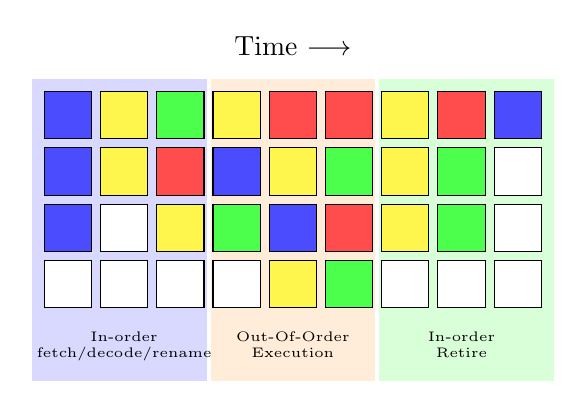
\begin{tikzpicture}[scale=0.5,
    T0/.style={fill=blue!70},
    T1/.style={fill=yellow!70},
    T2/.style={fill=green!70},
    T3/.style={fill=red!70},
    empty/.style={fill=white}]
    \matrix[matrix of nodes,
        nodes={draw=black, minimum size=6mm, anchor=center},
        column sep=1mm, row sep=1mm,
        ampersand replacement=\&] (m) {
        |[T0]| \phantom{X} \& |[T1]| \phantom{X} \& |[T2]| \phantom{X} \& |[T1]| \phantom{X} \& |[T3]| \phantom{X} \& |[T3]| \phantom{X} \& |[T1]| \phantom{X} \& |[T3]| \phantom{X} \& |[T0]| \phantom{X} \\
        |[T0]| \phantom{X} \& |[T1]| \phantom{X} \& |[T3]| \phantom{X} \& |[T0]| \phantom{X} \& |[T1]| \phantom{X} \& |[T2]| \phantom{X} \& |[T1]| \phantom{X} \& |[T2]| \phantom{X} \& |[empty]| \phantom{X} \\
        |[T0]| \phantom{X} \& |[empty]| \phantom{X} \& |[T1]| \phantom{X} \& |[T2]| \phantom{X} \& |[T0]| \phantom{X} \& |[T3]| \phantom{X} \& |[T1]| \phantom{X} \& |[T2]| \phantom{X} \& |[empty]| \phantom{X} \\
        |[empty]| \phantom{X} \& |[empty]| \phantom{X} \& |[empty]| \phantom{X} \& |[empty]| \phantom{X} \& |[T1]| \phantom{X} \& |[T2]| \phantom{X} \& |[empty]| \phantom{X} \& |[empty]| \phantom{X} \& |[empty]| \phantom{X} \\
    };
    \node[above=2mm of m.north] {Time $\longrightarrow$};

    % Pipeline stage labels (as nodes for positioning)
    \node[font=\tiny, align=center, text depth=0.5ex] (label1) at ([yshift=-10mm]$(m-4-1.south)!0.5!(m-4-3.south)$) {In-order\\fetch/decode/rename};
    \node[font=\tiny, align=center, text depth=0.5ex] (label2) at ([yshift=-10mm]$(m-4-4.south)!0.5!(m-4-6.south)$) {Out-Of-Order\\Execution};
    \node[font=\tiny, align=center, text depth=0.5ex] (label3) at ([yshift=-10mm]$(m-4-7.south)!0.5!(m-4-9.south)$) {In-order\\Retire};

    % Common bottom coordinate for all backgrounds
    \coordinate (bgbottom) at ([yshift=-2mm]label1.south);

    % Background shading for pipeline stages (behind the matrix, extending to labels)
    \begin{scope}[on background layer]
        \fill[blue!15] ([xshift=-3mm,yshift=3mm]m-1-1.north west) rectangle ([xshift=0.5mm]m-4-3.south east |- bgbottom);
        \fill[orange!15] ([xshift=-0.5mm,yshift=3mm]m-1-4.north west) rectangle ([xshift=0.5mm]m-4-6.south east |- bgbottom);
        \fill[green!15] ([xshift=-0.5mm,yshift=3mm]m-1-7.north west) rectangle ([xshift=3mm]m-4-9.south east |- bgbottom);
    \end{scope}
\end{tikzpicture}
\end{center}

\begin{alertblock}{Key Benefit}
Increases utilization/throughput by reducing impact of dependencies, cache misses, and branch mispredictions
\end{alertblock}
\end{frame}

\section{Performance Analysis}

\subsection{Question 1: Switch-on-Event Analysis}

\begin{frame}{Q1: Switch-on-Event Analysis}
\textbf{Given Parameters:}
\begin{itemize}
    \item Every M-th instruction is a memory access
    \item Memory access takes Q cycles
    \item Thread switch cost is zero
    \item Given $CPI_{ideal}$
    \item N threads available
\end{itemize}

\vspace{2mm}
\begin{center}
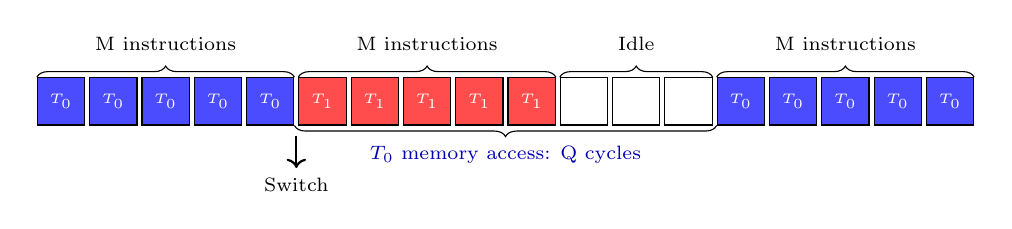
\begin{tikzpicture}[scale=0.45,
    T0/.style={fill=blue!70, text=white, font=\tiny\bfseries},
    T1/.style={fill=red!70, text=white, font=\tiny\bfseries},
    empty/.style={fill=white},
    bracelabel/.style={font=\scriptsize, text depth=0.5ex}]
    \matrix[matrix of nodes,
        nodes={draw=black, minimum size=6mm, anchor=center},
        column sep=0.5mm, row sep=0mm,
        ampersand replacement=\&] (m) {
        |[T0]| $T_0$ \& |[T0]| $T_0$ \& |[T0]| $T_0$ \& |[T0]| $T_0$ \& |[T0]| $T_0$ \&
        |[T1]| $T_1$ \& |[T1]| $T_1$ \& |[T1]| $T_1$ \& |[T1]| $T_1$ \& |[T1]| $T_1$ \&
        |[empty]| \phantom{X} \& |[empty]| \phantom{X} \& |[empty]| \phantom{X} \&
        |[T0]| $T_0$ \& |[T0]| $T_0$ \& |[T0]| $T_0$ \& |[T0]| $T_0$ \& |[T0]| $T_0$ \\
    };

    % Braces and labels above for execution
    \draw[decorate, decoration={brace, amplitude=4pt}]
        (m-1-1.north west) -- (m-1-5.north east)
        node[midway, above=4pt, bracelabel] {M instructions};
    \draw[decorate, decoration={brace, amplitude=4pt}]
        (m-1-6.north west) -- (m-1-10.north east)
        node[midway, above=4pt, bracelabel] {M instructions};
    \draw[decorate, decoration={brace, amplitude=4pt}]
        (m-1-11.north west) -- (m-1-13.north east)
        node[midway, above=4pt, bracelabel] {Idle};
    \draw[decorate, decoration={brace, amplitude=4pt}]
        (m-1-14.north west) -- (m-1-18.north east)
        node[midway, above=4pt, bracelabel] {M instructions};

    % Brace below for Q cycles (memory access time for T_0)
    \draw[decorate, decoration={brace, amplitude=4pt, mirror}]
        (m-1-5.south east) -- (m-1-14.south west)
        node[midway, below=4pt, bracelabel, blue!70!black] {$T_0$ memory access: Q cycles};

    % Switch on event arrow
    \draw[->, thick] ([yshift=-3mm]$(m-1-5.south)!0.5!(m-1-6.south)$) -- ([yshift=-12mm]$(m-1-5.south)!0.5!(m-1-6.south)$)
        node[below, font=\scriptsize] {Switch};
\end{tikzpicture}
\end{center}
\end{frame}

\begin{frame}{Q1a: IPC Equation Development}
\textbf{Question:} Develop an equation for IPC as a function of running threads (N)

\pause
\vspace{3mm}

\begin{block}{CPI per Thread}
$$CPI_{Thread} = CPI_i + \frac{Q}{M}$$
\end{block}

Where:
\begin{itemize}
    \item $CPI_i$ = ideal CPI
    \item Q = memory access cycles
    \item M = instructions between memory accesses
\end{itemize}

\begin{alertblock}{IPC Formula}
$$IPC = \frac{N}{CPI_i + \frac{Q}{M}}$$
\end{alertblock}
\end{frame}

\begin{frame}{Q1b: Best Achievable Performance}
\textbf{Question:} What is the best achievable performance?

\pause
\vspace{2mm}

\textbf{Maximum IPC when memory latencies are fully hidden:}
\begin{itemize}
    \item Achieved when all latencies are masked by other threads
\end{itemize}

\begin{center}
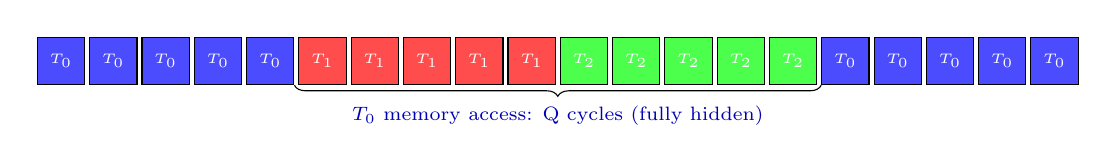
\begin{tikzpicture}[scale=0.45,
    T0/.style={fill=blue!70, text=white, font=\tiny\bfseries},
    T1/.style={fill=red!70, text=white, font=\tiny\bfseries},
    T2/.style={fill=green!70, text=white, font=\tiny\bfseries},
    bracelabel/.style={font=\scriptsize, text depth=0.5ex}]
    \matrix[matrix of nodes,
        nodes={draw=black, minimum size=6mm, anchor=center},
        column sep=0.5mm, row sep=0mm,
        ampersand replacement=\&] (m) {
        |[T0]| $T_0$ \& |[T0]| $T_0$ \& |[T0]| $T_0$ \& |[T0]| $T_0$ \& |[T0]| $T_0$ \&
        |[T1]| $T_1$ \& |[T1]| $T_1$ \& |[T1]| $T_1$ \& |[T1]| $T_1$ \& |[T1]| $T_1$ \&
        |[T2]| $T_2$ \& |[T2]| $T_2$ \& |[T2]| $T_2$ \& |[T2]| $T_2$ \& |[T2]| $T_2$ \&
        |[T0]| $T_0$ \& |[T0]| $T_0$ \& |[T0]| $T_0$ \& |[T0]| $T_0$ \& |[T0]| $T_0$ \\
    };

    % Brace below for Q cycles (memory access time for T_0)
    \draw[decorate, decoration={brace, amplitude=4pt, mirror}]
        (m-1-5.south east) -- (m-1-16.south west)
        node[midway, below=4pt, bracelabel, blue!70!black] {$T_0$ memory access: Q cycles (fully hidden)};
\end{tikzpicture}
\end{center}

\begin{alertblock}{Maximum IPC}
$$IPC_{Max} = IPC_{ideal}$$
\end{alertblock}
\end{frame}

\begin{frame}{Q1c: Minimum Threads for Maximum Performance}
\textbf{Question:} How many threads are needed to achieve maximum performance?

\pause
\vspace{3mm}

Starting from the IPC equation:
\vspace{-8mm}
$$IPC = \frac{N}{CPI_i + \frac{Q}{M}}$$

For maximum performance, $IPC = IPC_{ideal} = \frac{1}{CPI_i}$:
$$\frac{1}{CPI_i} = \frac{N1}{CPI_i + \frac{Q}{M}}$$

Solving for $N1$:
\vspace{-3mm}
$$CPI_i + \frac{Q}{M} = N1 \cdot CPI_i$$

\begin{alertblock}{Minimum Threads}
$$N1 = 1 + \frac{Q}{M \cdot CPI_i}$$
\end{alertblock}
\end{frame}

\subsection{Question 2: IPC vs Number of Threads}

\begin{frame}{Q2: IPC vs Number of Threads}
\textbf{Question:} Draw a graph of IPC as a function of number of threads (N)

\pause
\begin{center}
\begin{tikzpicture}[scale=0.8]
    \draw[->] (0,0) -- (8,0) node[right] {N = Threads};
    \draw[->] (0,0) -- (0,4.5) node[above] {IPC};
    
    % Draw roofline (not curve)
    \draw[thick, blue] (0,0) -- (3,3.5);
    \draw[thick, blue] (3,3.5) -- (7.5,3.5);
    
    % Mark key points
    \draw[dashed] (3,0) -- (3,3.5) node[pos=0, below] {$N_1$};
    \draw[dashed] (0,3.5) -- (3,3.5) node[pos=0, left] {$IPC_{Max}$};
    
    % Equation annotation
    \node at (5.5,2) {$IPC = \frac{N}{CPI_i + \frac{Q}{M}}$};
\end{tikzpicture}
\end{center}
\end{frame}

\section{Cache Impact}

\subsection{Question 3: Cache Analysis}

\begin{frame}{Q3a: L1 Cache Addition}
\textbf{Improvement Proposal:} Add L1 cache with 0 cycles access time

\textbf{Modified IPC with Cache:}
$$IPC = \frac{N}{CPI_i + k \cdot \frac{Q}{M}} \quad \text{where } k = \text{miss rate (k = 1} \rightarrow \text{100\% miss rate)}$$

\textbf{Question:} What cache hit rate provides maximum performance with $N_1/2$ threads?
\begin{align*}
IPC_{Max} &= IPC_{ideal} & \Rightarrow N_1 = 1 + \frac{Q}{M \cdot CPI_i} \quad \Rightarrow \quad \frac{N_1}{2} = \frac{1 + \frac{Q}{M \cdot CPI_i}}{2}
\end{align*}

Solve: $IPC\Big|_{N=\frac{N_1}{2}} = \left(CPI_i + k \cdot \frac{Q}{M}\right)^{-1} \cdot \frac{1}{2} \cdot CPI_i^{-1} = CPI_i^{-1}$

\begin{tcolorbox}[colback=blue!5!white,colframe=blue!75!black]
$$CPI\left(\frac{N_1}{2}\right) = \left(CPI_i + Q \cdot \frac{k}{M}\right) \cdot \frac{2 \cdot M \cdot CPI_i}{M \cdot CPI_i + Q} = CPI_i$$
\end{tcolorbox}

\alert{Result: $k = 0.5$ (50\% miss rate) $\Rightarrow$ 50\% hit rate required}
\end{frame}

\begin{frame}{Q3b: Cache Design Impact}
\textbf{How will cache addition affect the CPU?}

\begin{columns}
\column{0.30\textwidth}
\begin{block}{Area}
\textcolor{red}{Increase} \\
Cache requires silicon area
\end{block}

\column{0.30\textwidth}
\begin{block}{Power}
\textcolor{green}{Decrease} \\
(with sufficient hit rate)
\end{block}

\column{0.33\textwidth}
\begin{block}{Complexity}
\textcolor{red}{Increase} \\
Cache control logic needed
\end{block}
\end{columns}

\vspace{0.5cm}
\begin{itemize}
    \item Might allow CPU redesign with fewer threads if hit rate is high enough
\end{itemize}
\end{frame}


\section{Power/Performance Trade-offs}

\subsection{Question 4: Power/Performance Analysis}

\begin{frame}{Q4a: Single Thread Performance}
\textbf{Question:} Which processor provides best single-thread performance at 4W?

\begin{columns}[t]
\column{0.48\textwidth}
\textbf{Two Processor Options:}
\vspace{-2mm}
\begin{table}
\centering
\scriptsize
\begin{tabular}{lcc}
\toprule
Parameter & Small & Large \\
\midrule
Area & 2 mm² & 4 mm² \\
Width & 2-wide & 4-wide \\
IPC & 1 & 2 \\
Leakage & 0.5W & \textcolor{red}{\textbf{?}} \\
Cap. & 500 pF & 1500 pF \\
Threads & 1 & 1 \\
\bottomrule
\end{tabular}
\end{table}

\column{0.48\textwidth}
\textbf{Voltage-Frequency Points:}
\vspace{-2mm}
\begin{table}
\centering
\scriptsize
\begin{tabular}{ccc}
\toprule
V (V) & Large & Small \\
\midrule
0.6 & 0.7 & 1.0 \\
0.65 & 1.0 & 1.25 \\
0.7 & 1.35 & 1.5 \\
0.75 & 1.75 & 1.75 \\
0.8 & 2.25 & 2.0 \\
0.85 & 2.5 & 2.25 \\
0.9 & 3.0 & 2.5 \\
0.95 & 3.5 & 2.75 \\
1.0 & 4.0 & 3.0 \\
\bottomrule
\end{tabular}
\end{table}
\end{columns}

\begin{block}{Key Assumption}
Leakage is approximately proportional to area
\end{block}
\end{frame}

\begin{frame}{Q4a: Leakage Power Calculation}
\textbf{Question:} Which processor provides best single-thread performance at 4W?

\textbf{First, we compute the leakage power for the large core:}

\begin{columns}
\column{0.5\textwidth}
\begin{table}
\centering
\small
\begin{tabular}{lcc}
\toprule
Parameter & Small & Large \\
\midrule
\rowcolor{yellow!30} Area & 2 mm² & 4 mm² \\
Width & 2-wide & 4-wide \\
IPC & 1 & 2 \\
\rowcolor{yellow!30} Leakage & 0.5W & \textcolor{red}{\textbf{?}} \\
Cap. & 500 pF & 1500 pF \\
Threads & 1 & 1 \\
\bottomrule
\end{tabular}
\end{table}

\column{0.5\textwidth}
\begin{alertblock}{General Formula}
$$\text{Leakage} \propto \text{Area}$$
\end{alertblock}

\textbf{For this question:}
$$\text{Leakage}_{\text{large}} = \frac{\text{area}_{\text{large}}}{\text{area}_{\text{small}}} \times \text{Leakage}_{\text{small}}$$

$$= \frac{4\text{ mm}^2}{2\text{ mm}^2} \times 0.5\text{W} = 1\text{W}$$
\end{columns}
\end{frame}

\begin{frame}{Q4a: Frequency Calculation (4W Budget)}
\textbf{Second, we compute the maximum frequency given the 4W power budget:}

\begin{columns}[t]
\column{0.35\textwidth}
\vspace{-3mm}
\begin{table}
\centering
\tiny
\begin{tabular}{lcc}
\toprule
Parameter & Small & Large \\
\midrule
Leakage & \cellcolor{yellow!40}0.5W & \cellcolor{green!25}1W \\
Cap. & \cellcolor{yellow!60!orange!40}500 pF & \cellcolor{green!40!cyan!30}1500 pF \\
\bottomrule
\end{tabular}
\end{table}

\vspace{1mm}

{\centering\tiny\textbf{Voltage-Frequency (GHz):}\par}
\vspace{0mm}

\begin{table}
\centering
\tiny
\begin{tabular}{ccc}
\toprule
V (V) & Small & Large \\
\midrule
0.6 & 1.0 & 0.7 \\
0.65 & 1.25 & 1.0 \\
0.7 & 1.5 & 1.35 \\
0.75 & 1.75 & 1.75 \\
0.8 & 2.0 & 2.25 \\
\cellcolor{cyan!35}0.85 & 2.25 & \cellcolor{cyan!50}2.5 \\
0.9 & 2.5 & 3.0 \\
0.95 & 2.75 & 3.5 \\
\cellcolor{orange!40}1.0 & \cellcolor{orange!60}3.0 & 4.0 \\
\bottomrule
\end{tabular}
\end{table}

\column{0.65\textwidth}
\vspace{-3mm}
\begin{alertblock}{Power Equation}
$$P = \text{Leakage} + C \cdot V^2 \cdot f$$
\end{alertblock}

\textbf{Small core:}
$4W \geq \colorbox{yellow!40}{0.5W} + \colorbox{yellow!60!orange!40}{500\text{pF}} \cdot V^2 \cdot f$\par
From table: $V = \colorbox{orange!40}{1\text{V}}$, $f = \colorbox{orange!60}{3\text{GHz}}$\par
\vspace{-4mm}
$$P = \colorbox{yellow!40}{0.5} + \colorbox{yellow!60!orange!40}{500} \cdot \colorbox{orange!40}{1}^2 \cdot \colorbox{orange!60}{3} = 2\text{W} < 4\text{W} \checkmark$$

\textbf{Large core:}
$4W \geq \colorbox{green!25}{1W} + \colorbox{green!40!cyan!30}{1500\text{pF}} \cdot V^2 \cdot f$\par
From table: $V = \colorbox{cyan!35}{0.85\text{V}}$, $f = \colorbox{cyan!50}{2.5\text{GHz}}$\par
\vspace{-4mm}
$$P = \colorbox{green!25}{1} + \colorbox{green!40!cyan!30}{1500} \cdot \colorbox{cyan!35}{0.85}^2 \cdot \colorbox{cyan!50}{2.5} = 3.7\text{W} < 4\text{W} \checkmark$$
\end{columns}
\end{frame}

\begin{frame}{Q4a: Performance Comparison}
\textbf{Finally, we compare the performance:}

\begin{block}{Performance Metric}
$$\text{Performance} \propto \text{IPC} \times \text{Frequency}$$
\end{block}

\textbf{Given:} Small core IPC = 1, Large core IPC = 2

\textbf{Results:}
\begin{itemize}
    \item \textbf{Small core:} IPC = 1, Frequency = 3 GHz
    $$\text{Performance} = 1 \times 3 = 3 \text{ G inst/sec}$$

    \item \textbf{Large core:} IPC = 2, Frequency = 2.5 GHz
    $$\text{Performance} = 2 \times 2.5 = 5 \text{ G inst/sec}$$
\end{itemize}

\alert{Result: Large core provides better performance (5 vs 3 G inst/sec)}
\end{frame}

\begin{frame}{Q4b: Multi-Thread Performance}
\textbf{Question:} Given a 2W power budget per core, which configuration provides best 2-way Multi-Thread performance: two large cores or two small cores?

\pause

\vspace{5mm}

\textbf{Approach:}
\begin{itemize}
    \item Calculate power consumption for different voltage-frequency points
    \item Find maximum frequencies that fit within 2W budget
    \item Compare performance of configurations
\end{itemize}
\end{frame}

\begin{frame}{Q4b: Voltage-Frequency Analysis}
\textbf{Question:} Given a 2W power budget per core, which configuration provides best 2-way Multi-Thread performance: two large cores or two small cores?

\vspace{3mm}

\begin{columns}[t]
\column{0.3\textwidth}
\scriptsize
\begin{tabular}{|c|c|c|}
\hline
\makecell{Voltage \\ (V)} &
\makecell{Freq \\ Small \\ Core \\ (GHz)} &
\makecell{Freq \\ Large \\ Core \\ (GHz)} \\
\hline
0.6 & 1 & 0.7 \\
0.65 & 1.25 & 1 \\
0.7 & 1.5 & 1.35 \\
0.75 & 1.75 & 1.75 \\
0.8 & 2 & 2.25 \\
0.85 & 2.25 & 2.5 \\
0.9 & 2.5 & 3 \\
0.95 & 2.75 & 3.5 \\
1 & 3 & 4 \\
\hline
\end{tabular}

\column{0.7\textwidth}

\vspace{-2.4cm}
\textbf{Given:}
\begin{itemize}
    \item Voltage-frequency points for each core type
    \item Small core: Leakage = 0.5W, C = 500 pF
    \item Large core: Leakage = 1W, C = 1500 pF
\end{itemize}

\vspace{3mm}

Considering the voltage-frequency relationship, we can calculate:
$$P_{act} = C \cdot V^2 \cdot f$$
$$P_{tot} = P_{act} + \text{Leakage}$$
\end{columns}
\end{frame}

\begin{frame}{Q4b: Power Table Analysis (2W per Core)}
\textbf{Question:} Given a 2W power budget per core (and the table below), which configuration provides best 2-way Multi-Thread performance: two large cores or two small cores?
\vspace{3mm}
\begin{columns}[t]
\column{0.57\textwidth}
\scriptsize
\begin{tabular}{|c|c|c|c|c|c|c|}
\hline
\makecell{Voltage \\ (V)} &
\makecell{Freq \\ Small \\ Core \\ (GHz)} &
\makecell{Freq \\ Large \\ Core \\ (GHz)} &
\makecell{$P_{act}$ \\ Small \\ Core \\ (W)} &
\makecell{$P_{act}$ \\ Large \\ Core \\ (W)} &
\makecell{$P_{tot}$ \\ Small \\ Core \\ (W)} &
\makecell{$P_{tot}$ \\ Large \\ Core \\ (W)} \\
\hline
0.6 & 1 & 0.7 & 0.18 & 0.38 & 0.68 & 1.38 \\
0.65 & 1.25 & 1 & 0.26 & 0.63 & 0.76 & 1.63 \\
0.7 & 1.5 & \only<2->{\cellcolor{cyan!40}}1.35 & 0.37 & 0.99 & 0.87 & \only<2->{\cellcolor{green!40}}1.99 \\
0.75 & 1.75 & 1.75 & 0.49 & 1.48 & 0.99 & 2.48 \\
0.8 & 2 & 2.25 & 0.64 & 2.16 & 1.14 & 3.16 \\
0.85 & 2.25 & 2.5 & 0.81 & 2.71 & 1.31 & 3.71 \\
0.9 & 2.5 & 3 & 1.01 & 3.65 & 1.51 & 4.65 \\
0.95 & 2.75 & 3.5 & 1.24 & 4.74 & 1.74 & 5.74 \\
1 & \only<2->{\cellcolor{yellow!50}}3 & 4 & 1.50 & 6.00 & \only<2->{\cellcolor{orange!50}}2.00 & 7.00 \\
\hline
\end{tabular}

\column{0.43\textwidth}

\vspace{-2.4cm}
\textbf{Answer:}

\vspace{2mm}

First, find $P_{act}$ and $P_{tot}$ based on the known leakage:

\vspace{1mm}

$P_{act} = C \cdot V^2 \cdot f$ \\
$P_{tot} = P_{act} + \text{Leakage}$

\pause

Then, find frequencies that fit within the 2W power budget per core:

\pause

\textbf{Small cores:} \colorbox{yellow!50}{3} GHz (\colorbox{orange!50}{2}W) \\
\textbf{Large cores:} \colorbox{cyan!40}{1.35} GHz (\colorbox{green!40}{1.99}W)
\end{columns}
\end{frame}

\begin{frame}{Q4b: Performance Calculation}
\textbf{Question:} Given a 2W power budget per core, which configuration provides best 2-way Multi-Thread performance: two large cores or two small cores?

\vspace{5mm}

\begin{block}{Performance Formula}
$$\text{Performance} = N \times F \times \text{IPC}$$
where $N$ = number of cores, $F$ = frequency, IPC = instructions per cycle
\end{block}

\vspace{5mm}

\textbf{Two Small cores:} $\text{Performance} = 2 \times 3\text{ GHz} \times 1 = 6 \text{ G inst/sec}$

\textbf{Two Large cores:} $\text{Performance} = 2 \times 1.35\text{ GHz} \times 2 = 5.4 \text{ G inst/sec}$

\vspace{5mm}

\alert{Result: Two small cores provide better performance (6 vs 5.4 G inst/sec)}
\end{frame}

\begin{frame}{Power Curve Characteristics}
\begin{columns}
\column{0.45\textwidth}
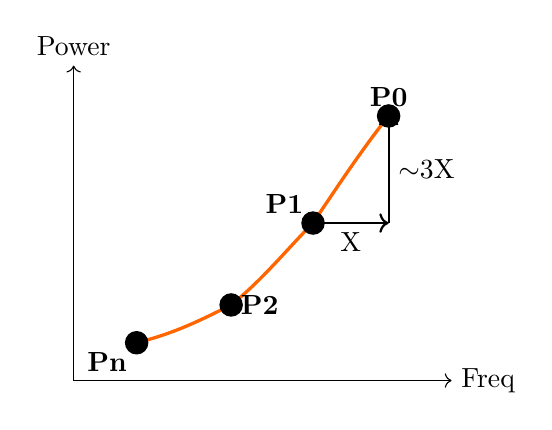
\begin{tikzpicture}[scale=0.8]
    \draw[->] (0,0) -- (6,0) node[right] {Freq};
    \draw[->] (0,0) -- (0,5) node[above] {Power};

    % Define point coordinates
    \coordinate (Pn) at (1,0.6);
    \coordinate (P2) at (2.5,1.2);
    \coordinate (P1) at (3.8,2.5);
    \coordinate (P0) at (5,4.2);

    % Draw curved segments between points (orange/red)
    \draw[thick, orange!80!red, line width=1.2pt] (Pn) .. controls (1.6,0.75) and (2,0.95) .. (P2);
    \draw[thick, orange!80!red, line width=1.2pt] (P2) .. controls (3,1.6) and (3.4,2.1) .. (P1);
    \draw[thick, orange!80!red, line width=1.2pt] (P1) .. controls (4.2,3.1) and (4.6,3.7) .. (P0);

    % Mark points with black circles
    \foreach \p in {Pn,P2,P1,P0} {
        \node[circle,fill=black,inner sep=3pt] at (\p) {};
    }

    % Labels for points
    \node[below left] at (Pn) {\textbf{Pn}};
    \node[right] at (P2) {\textbf{P2}};
    \node[above left] at (P1) {\textbf{P1}};
    \node[above] at (P0) {\textbf{P0}};

    % Horizontal arrow (X) from P1 rightward, vertical arrow (~3X) up to P0
    \draw[->,thick] (P1) -- (P0 |- P1);
    \node[below] at ($(P1)!0.5!(P0 |- P1)$) {X};
    \draw[->,thick] (P0 |- P1) -- (P0);
    \node[right] at ($(P0 |- P1)!0.5!(P0)$) {$\sim$3X};
\end{tikzpicture}

\column{0.55\textwidth}
\textbf{At $P_n$ ($V_{min}$ = Energy efficient point):}
\begin{itemize}\small
    \item Freq decrease doesn't decrease V: $P \propto K \cdot F$
    \item Freq decrease by 1\% decreases power by 1\%
    \item Perf. features better than 1:1
\end{itemize}

\vspace{0.3cm}
\textbf{At $P_2$ (mid-range):}
\begin{itemize}\small
    \item Perf. features better than 1:3
    \item (1\% perf / less than 3\% power)
\end{itemize}

\vspace{0.3cm}
\textbf{Key relationships:}
\begin{itemize}\small
    \item $P = CV^2f$; $f = KV \Rightarrow P \propto f^3$
    \item $E = P \times t \Rightarrow E \propto f^2$
\end{itemize}
\end{columns}
\end{frame}

\begin{frame}{Summary}
\begin{itemize}
    \item \textbf{Multithreading} improves processor utilization
    \item \textbf{SMT} provides best resource utilization
    \item \textbf{IPC} increases with thread count up to saturation
    \item \textbf{Cache} can reduce required thread count
    \item \textbf{Power/Performance} trade-offs depend on workload:
    \begin{itemize}
        \item Single-thread: Large cores often better
        \item Multi-thread: Small cores can be more efficient
    \end{itemize}
    \item \textbf{Energy efficiency} achieved at moderate frequencies
\end{itemize}
\end{frame}

\end{document}